\documentclass[tikz,border=2pt]{standalone}
\usepackage{amsmath}
\usepackage{pgfplots}
\pgfplotsset{compat=1.18}

\begin{document}
% f(x) -> L as x -> +infinity: for every band L±ε there is an M beyond which the graph stays in it.
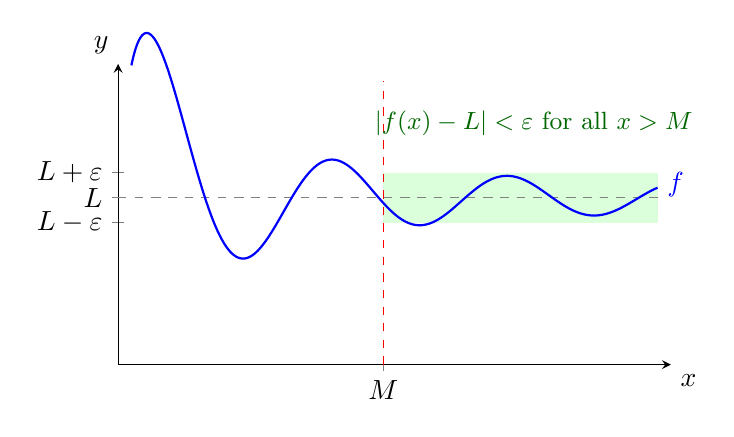
\begin{tikzpicture}
	\begin{axis}[
		axis lines=middle,
		xmin=0, xmax=12.5,
		ymin=0, ymax=3.6,
		xtick={6}, xticklabels={$M$},
		ytick={1.7,2,2.3}, yticklabels={$L-\varepsilon$,$L$,$L+\varepsilon$},
		xlabel={$x$}, ylabel={$y$},
		xlabel style={below right}, ylabel style={above left},
		samples=300, smooth, clip=false,
		width=8.6cm, height=5.4cm
		]
		\fill[green!14] (axis cs:6,1.7) rectangle (axis cs:12.2,2.3);
		\addplot[gray, dashed, domain=0:12.2] {2};
		\draw[dashed, red] (axis cs:6,0) -- (axis cs:6,3.4);
		\addplot[thick, blue, domain=0.3:12.2] {2+2.4*sin(deg(1.6*x))/(x+0.4)};
		\node[green!40!black, anchor=south, font=\small] at (axis cs:9.4,2.62) {$|f(x)-L|<\varepsilon$ for all $x>M$};
		\node[blue, anchor=west] at (axis cs:12.2,2.15) {$f$};
	\end{axis}
\end{tikzpicture}
\end{document}
